\section*{Источники и решения}

\subsubsection*{Любовь в Клептопии}

Этот вопрос приводится в книге Саймона Сингха \cite{53};
я узнал его от Кэролайн Калдербэнк, дочки пары математиков Ингрид Добеки и Роба Калдербэнка.
В решении Кэролайн, Ян отправляет Марии ящик с кольцом внутри, навесив на него один из своих замков.
По получении Мария навешивает свой собственный замок на ящик и отправляет его назад с обоими замками.
Когда Ян получает ящик, он снимает свой замок и отправляет ящик опять Марии --- вуаля!

Это решение не просто игра;
на нём основан обмен ключами шифрования в протоколе Мэсси --- Омуры, %Диффи — Хеллмана,
--- исторический прорыв в криптографии.

В зависимости от предположений, возможны и другие решения.
Моё любимое предложено компанией (включающей оригамиста Роберта Лэнга) на конференции
«Ga\-the\-ring for Gardner VII».
Яну надо найти замок, ключ от которого имеет большое отверстие, или по крайней мере, отверстие, которое может быть достаточно увеличено сверлением, чтобы ключ мог быть нацеплен за дужку другого замка.
Ян использует этот второй замок, с упомянутым ключом на его дужке, чтобы запереть пустой ящичек, который он отправляет Марии.
По прошествии времени, достаточном для пересылки (или возможно, после электронного подтверждения от Марии), он отправляет кольцо в другом ящике, запертой первым замком.
Получив ящик, Мария открывает его ключом, прикреплённым к первому ящичку, и забирает кольцо.

%\begin{addedbytheeditors}
%Последнее решение в криптографии иллюстрирует трёхэтапный протокол \cite{three-pass_protocol}, точнее %криптосистему Мэсси --- Омуры.\pr 
%%??? я не увидел связь с этим протоколом --- если она есть, то наверно стоит что-то о ней сказать.
%\end{addedbytheeditors}

% М.б. ""страна клептократов""?" --- А: кратия пахнет политикой (я против).

\subsubsection*{Черви и вода}

Эта головоломка скорее инженерная, чем математическая.
Она пришла ко мне от Балинта Вирага из Массачусетского технологического института.

Лори может защититься от червей свесив с потолка большой навес, выходящий далеко за кровать.
Но навес должен загибаться внутрь \emph{под себя}, создавая кольцевой жёлоб, заполненный водой.
(Поперечный разрез навеса показан на рис. \ref{pic:chervi}.)

\begin{figure}[h!]
\centering
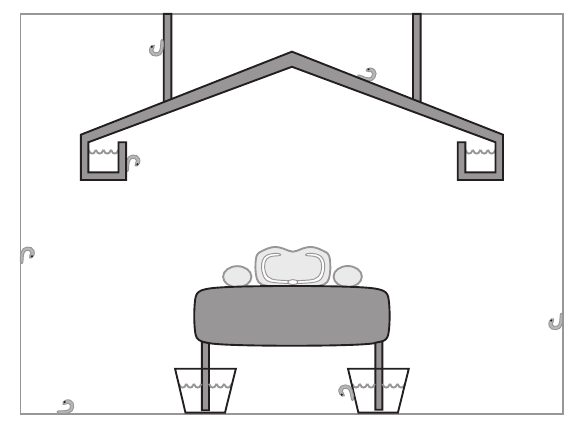
\includegraphics[scale=0.5]{pics/chervi}
\caption{Поперечный разрез Лори в защищённой от червей кровати.}
\label{pic:chervi}
\end{figure}

Если у червей нет способа проникнуть в спальню сверху, то Лори может защититься, обведя комнату по краю жёлобом с водой.

\begin{addedbytheeditors}
В рассказе Льва Толстого «Клопы» описывается та же задача, но с другим решением --- надеть шубу и выйти на двор.
\pr
\end{addedbytheeditors} 

\subsubsection*{Проверка страусиных яиц}

Вариант этой задачи появился в замечательной книге Джозефа Д. Э. Конхаузера, Дэна Веллемана и Стэна Вэгона \cite{42}.

Часто полезно считать данное число (в нашем случае 102) переменной, даже если в конечном счёте нас интересует лишь одно значение.
Пусть $f(k)$ --- максимальное число этажей, которые проверяются зане более чем за $k$ бросков, имея вначале два яйца.
Таким образом, $f(1) = 1$ (прочность яйца может быть $0$ или $1$).
Предположим, что Оскару разрешено сделать $k$ бросков, и он делает первый с $n$-го этажа.
Если яйцо разбилось, то Оскару придётся бросить единственное оставшееся яйцо с 1-го этажа, затем с 2-го и так далее до $(n-1)$-го в худшем случае;
так что $n = k$ это наилучший вариант.
Если яйцо пережило падение с $k$-го этажа, то придётся проверить все этажи выше оставшимися $k-1$ броском (используя два яйца).
Следовательно, $f(k - 1) + k$ это максимальное число этажей, которые можно обработать,
получаем рекурсию $f(k) = f(k - 1) + k$.

Прямым вычислением убеждаемся, что $f(2) = 3$, $f(3) = 6$, $f(5) = 10$ и так далее; в общем случае $f(k)$ равно сумме чисел от $1$ до $k$.
Поскольку таких чисел $k$, а их среднее равно $(k + 1)/2$, их сумма (иногда называемая \emph{$k$-м треугольным числом}), составляет $k(k + 1)/2$.
Первое значение $f(k)\ge 102$, это $f(14) \z= 14 \times 15/2 \z= 105$, то есть в худшем случае Оскару понадобится $14$ бросков.
Рекурсия указывает и на то как это сделать;
в нашем случае, трёхэтажный запас позволяет Оскару сбросить первое яйцо с одиннадцатого, двенадцатого, тринадцатого или четырнадцатого этажа.
Любой другой вариант может потребовать лишнего броска.

Давайте посмотрим, что происходит с тремя яйцами.
Определим $g(k)$ как максимальное число этажей, которые можно обработать $k$ бросками, имея три яйца.
Теперь Оскару нужно обработать $g(k \z- 1)$ этажей выше уровня первого броска, если яйцо переживёт падение;
или же $f(k - 1)$ этажей ниже этого уровня (то же $f$, что и выше), потому что в этом случае у него лишь два яйца.
Получаем новую рекурсию: $g(k) = g(k-1) + 1 + (k - 1)k/2$, что даёт $g(2) = 3$ (пока без улучшений), но $g(3) = 7$.
В общем случае $g(k)=k(k^2+5)/6$ и наименьшее значение $k$, для которого $g(k)\ge 102$, равно $9$.
То есть, если у Оскара три яйца, то ему потребуется максимум девять бросков для обработки всех этажей.

В общем случае, если $k$ велико, то число этажей, которые можно обработать, имея вначале $m$ яиц, равно $k^m/m!$ плюс члены низших порядков.
Отсюда следует, что с $m$ яйцами и небоскрёбом в $n$ этажей, при $n$ намного большем чем $m$, надо около $(m!\times n)^{1/m}$ бросков в худшем случае.

\subsubsection*{Ненадежная картина}

Эту интересную головоломку предложил Джулио Дженовезе, аспирант в Дартмуте, который узнал её из нескольких источников в Европе.

Один из способов повесить картину изображён на рис. \ref{pic:kartina2}, с зазором, чтобы было видно как идёт шнур.
Он проходит над первым гвоздём, далее идёт петля вокруг второго,
проходит опять над первым гвоздём, и затем снова петля вокруг второго гвоздя, но с подворотом.

\begin{figure}[h!]
\centering
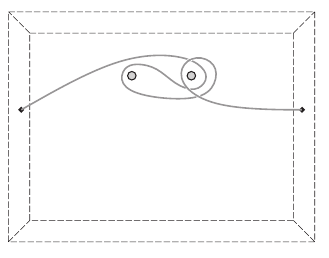
\includegraphics[scale=1]{pics/kartina2}
\caption{Эта картина упадёт если выпадет любой из двух гвоздей.}
\label{pic:kartina2}
\end{figure}

Существуют также некоторые нетопологические решения: например, можно сдавить петлю между двумя близко расположенными гвоздями, предполагая, что ширина головки гвоздя не намного больше толщины шнура.
Но зачем полагаться на трение, когда можно использовать математику?

\begin{addedbytheeditors}
Попробуйте повесить картину на $n$ гвоздей так, чтобы она упала если выпадет любой из них.
А можно ли повесить так, чтоб картина осталась висеть при выпадании одного гвоздя, но падала при выпадании двух?
Хороший обзор подобных задач дан в \cite{demaine2014}, но он не включает результата из \cite{gartside-greenwood}, дающего наилучший способ решения задачи с $n$ гвоздями (без заузливания шнура); см. также \cite{epifanov}.

Решение напоминает \emph{борромеевы кольца};
одно из колец следует считать шнурком, а два других соответсвуют гвоздям.
Для большего числа колец подобные конструкции называются \emph{зацеплениями Брунна}.
В комплексном анализе линия, образованная шнуром, называется контуром Похгаммера.
Она используется для записи специальных функций в виде контурных интегралов от многозначных функций (данные точки --- точки ветвления).
%Этот замкнутый путь обходит каждую из двух данных точек как по, так и против часовой стрелки.
%Чтобы решить задачу в общем случае, удобно перевести её на язык алгебры.
%Обозначим обход первой точки $A$ против часовой стрелки символом $a$, а обход по часовой стрелки -- символом $a^{-1}$.
%Если мы сделаем два таких обхода один за другим, то петля не зацепится за точку $A$ (в таком случае говорят, что петля может быть стянута в точку).
%В символическом виде это выражается формулой $aa^{-1}=1$.
%Обходы против часовой и по часовой стрелке вокруг точки $B$ обозначим соответственно символами $b$ и $b^{-1}$.
%Легко видеть, что пути $ab$ и $ba$ --- разные, то есть введённые нами переменные не коммутируют.
%Тот путь, который решает задачу, можно записать в виде $aba^{-1}b^{-1}$.
%Такое выражение называется коммутатором $a$ и $b$, и обозначается $[a,b]$.
%Убирание первого гвоздя можно понимать как присваивание переменной $a$ значения 1.
%В результате получаем, что $[a,b]=bb^[-1}=1$, то есть петля стягивается и картина падает.
%То же самое происходит, если убрать второй гвоздь (то есть положить $b=1$).
%Теперь становится понятно, как решать задачу в более общем случае.
%Например, есди гвоздей три, то решением будет контур, который имеет вид $[[a,b],c]$.
%Проверьте, что это выражение действительно будет равно единице, если любой из трёх переменных присвоить единичное значение.
\end{addedbytheeditors}

\subsubsection*{Замок с дефектом}

Этот комбинаторный шедевр достался мне от Амит Чакрабарти из Дартмута;
он был предложен ГДР для Международной математической олимпиады 1988 года.

Задачи такого рода лучше решать геометрически.
Пространство всех комбинаций представляет собой комбинаторный куб $8 \times 8 \times 8$.
Каждый раз, когда мы проверяем какую-то точку куба, мы вычёркиваем все точки на трёх её координатных линиях.

Представив задачу таким образом, легче увидеть, что лучший способ вычеркнуть все точки --- это брать все тестовые точки в двух противоположных осьмушках $4 \times 4 \times 4$ нашего куба.
Так можно догадаться до следующего решения.

Проверим все комбинации с числами из $\{1, 2, 3, 4\}$, сумма которых кратна $4$.
Их всего шестнадцать, ведь если выбирать числа на первых двух (или любых двух) дисках, то число на третьем определяется однозначно.
Теперь попробуем те же комбинации, добавив $(4,4,4)$, то есть, добавив по $4$ к каждому из трёх чисел;
их ещё $16$, и мы утверждаем, что вместе эти $32$ тестовые комбинации вычёркивают все.

Это несложно проверить.
У правильной комбинации либо два (или более) числа из $\{1, 2, 3, 4\}$, либо два числа из  $\{5, 6, 7, 8\}$.
В первом случае положение третьего диска единственно (это число в правильной комбинации может не входить в $\{1, 2, 3, 4\}$), так что получена тройка среди первых $16$ тестовых комбинаций.
Второй случай аналогичен.

А вот способ Амита (есть и другие), объясняющий, что нельзя обойтись $31$-й или менее тестовой комбинацией.
Предположим, что $S$ --- набор из 31-й точки, который всё покрывает.
Пусть $S_i = \{\,(x, y, z) \z\in S : z = i\,\}$ будет $i$-м уровнем $S$.

Рассмотрим три множества:
$A=\{1, 2, 3\}$,
$B = \{4, 5, 6, 7, 8\}$,
и $C \z= \{2, 3, 4, 5, 6, 7, 8\}$.
По крайней мере, один уровень $S$ должен содержать три или меньше точек;
можно считать, что это $S_1$, и $|S_1| = 3$.
(Если $|S_1| \le 2$, то прийти к противоречию ещё проще.)
Точки $S_1$ должны лежать в некотором $3 \times 3 \times 1$ подкубе;
можно считать, что они лежат в $A \times A \times {1}$.

$25$ точек из $B \times B \times \{1\}$ должны быть вычеркнуты тестовыми точками, не входящими в $S_1$.
Никакие две из них не могут быть вычеркнуты одной точкой в $S$.
Следовательно, $S - S_1$ содержит подмножество $T$ размером $25$, которое лежит в подкубе $B \times B \times C$.
Теперь рассмотрим множество $P = \{\,(x, y, z) : z \in C, (x, y, 1) \notin S_1 , (x, y) \notin B \times B\,\}$.
Легко убедиться, что $|P| = (64-3-25) \times 7 = 252$.
Точки в $P$ не вычёркиваются посредством $S_1$, и каждая точка в $T$ может вычеркнуть не более $3 + 3 = 6$ точек в $P$. Следовательно, есть по крайней мере $252 - 6 \times 25 = 102$ точки в $P$, которые должны быть вычеркнуты точками в $S - S_1 - T$.

Однако осталось всего $|S - S_1 - T | = 31 - 3 - 25 = 3$ тестовые точки, и каждая из них вычёркивает ровно $22$ точки.
Поскольку $22 \times 3 = 66 \z< 102$, приходим к противоречию. 

\subsubsection*{Альтернативные кубики}

Эта задача настолько известна, что имеет собственное название: «кубики Зихермана».
В заметке Мартина Гарднера 1978 года \cite{25} или в его книге \cite{28} можно узнать об их открытии полковником Джорджем Зихерманом, сейчас проживающим в штате Нью-Джерси.%
\footnote{На веб-сайте автора есть страница про эти кубики \cite{sicherman}.}
Единственная пара кубиков Зихермана имеет метки $\{1$, $3$, $4$, $5$, $6$, $8\}$ и $\{1$, $2$, $2$, $3$, $3$, $4\}$.

Возможно, вы нашли ответ перебором, что вполне приемлемо.
Однако есть и другой способ, иллюстрирующий мощный математический инструмент --- \emph{производящие функции}.

Идея сопоставить кубику многочлен от переменной $x$, в котором коэффициент при $x^k$ равен числу граней кубика с меткой $k$.
Обычный кубик, например, будет соответствовать многочлену 
\[f(x) \z= x \z+ x^2 \z+ x^3 \z+ x^4 \z+ x^5 \z+ x^6.\]

Важно заметить, что результат броска двух (или более) кубиков соответствует \emph{произведению} их многочленов.
Например, если мы бросаем два обычных кубика, то коэффициент при $x^{10}$ в произведении (то есть в $f(x)^2$) есть число способов выбрать два члена из $f(x)$, произведение которых равно $x^{10}$ ---
это $x^4 \times x^6$, $x^5 \times x^5$ и $x^6 \times x^4$; они и представляют три способа получить в сумме $10$.

Следовательно, если $g(x)$ и $h(x)$ --- многочлены наших кубиков, то $g(x) \times h(x) = f(x)^2$.
Многочлены, как и числа, разлагаются единственным способом на простые сомножители;
многочлен $f(x)$ разлагается как $x(x + 1)(x^2 + x + 1)(x^2 - x + 1)$.
Чтобы получить произведение $g(x)$ и $h(x)$ равное $f(x)^2$, надо взять каждый из этих $4$ сомножителей и добавить по одной его копии в $g(x)$ и в $h(x)$, или же две его копии в один либо в другой.
При этом есть следующие ограничения:
в полученных многочленах $g(x)$ и $h(x)$ не может быть свободных членов (это бы означало, что некоторые стороны помечены нулём);
не допускаются отрицательные коэффициенты;
также сумма коэффициентов в каждом из многочленов равна 6-ти.


Единственное решение (кроме $g(x) = h(x) = f(x)$) это
\begin{align*}
g(x)
&=
x(x + 1)(x^2 + x + 1)
=
\\
&=
x + 2x^2 + 2x^3 + x^4
\intertext{и}
h(x)
&=
x(x + 1)(x^2 + x + 1)(x^2 - x + 1)^2
=
\\
&=
x + x^3 + x^4 + x^5 + x^6 + x^8,
\end{align*}
или наоборот.

Это всё ещё перебор, но так решаются задачи посложнее.
Во-первых, можно придумать альтернативы для пары восьмигранных игральных костей, пронумерованных от $1$ до $8$ (есть три альтернативных варианта), или для бросания \emph{трёх} обычных кубиков (много способов).

Тем, кто хочет поглубже изучить эту тему, стоит обратиться к отличной статье Джо Галлиана и Дейва Русина \cite{22}.

\subsubsection*{Совпадение монет}

Эту задачу подкинул мне Одед Регев из Техниона (Израиль).

Сонни и Шер могут выиграть более чем в 2/3 случаев.
Для этого разделим последовательность бросков на блоки по три.
Перед каждым блоком Шер \emph{оповещает} Сонни, будут ли в следующем блоке в основном орлы или решки;
если первое, Сонни говорит «ООО» в этом блоке; если второе, то «РРР».

Но как Шер передать эту информацию?
Чаще всего Сонни придётся ошибаться (в точности) 1 раз в блок.
Перед этим броском Шер говорит «О», сообщая, что в следующем блоке будут в основном орлы, и «Р» в противном случае.
Для двух других бросков в текущей тройке Шер даёт правильный ответ (вместе с Сонни), гарантируя две из трёх побед.
Если случится, что Сонни может угадать все три броска в текущей тройке,
то один раз --- скажем на последнем броске, Шер действует, как описано выше, даже если это стоит одной победы.
Таким образом, после первого блока Сонни и Шер будут набирать две победы из трёх, когда блок состоит из двух орлов и одной решки или двух решек и одного орла.
Когда блок состоит полностью из орлов или полностью из решек (что происходит с вероятностью 1/4), они получают две победы из трёх в половине случаев и три из трёх в оставшейся половине.
И доля успеха составит $3/4 \times 2/3 + 1/4 \times 5/6 = 17/24 > 70.8\%$.
Обратите внимание, что даже в наихудшем случае (например, если последовательные орлы и решки выбираются противником, а не случайны) этот метод гарантирует $2/3$-и побед.

Оливье Госснер, Пенелопа Эрнандес и Абрахам Нейман \cite{32} доказали, что с более сложными версиями этой схемы Сонни и Шер могут приблизиться к любой доле успеха равной $x$, где $x$ --- единственное решение уравнения
\[-x \log_2 x - (1 - x) \log_2 (1 - x) + (1 - x) \log_2 3 = 1,\]
и лучшего добиться нельзя.
Более того, это утверждение остаётся верным независимо от того, случайны броски монеты или нет!
Это значение $x$ составляет около $0{,}8016$, то есть Сонни и Шер могут добиться  $80$-и процентов побед, даже если играют против них, зная их стратегию.

\begin{addedbytheeditors}
Илья Межиров предложил следующую схему с 80\%-ным успехом.

Вся серия бросков разбивается на блоки длины $5k$; значение $k$ уточним позднее.
Шер использует первый блок только чтобы сообщить Сонни, как ходить в следующем блоке.
В каждом из следующих блоков Шер будет знать все $5k$ битов и ходы Сонни,
однако ровно в $k$ битах они сделают ошибку по плану Шер. 

Заметим, что есть три вида ошибки (неугадывания бита): 
\begin{itemize}
\item Шер называет решку, а Сонни --- орла;
\item Шер называет орла, а Сонни --- решку;
\item оба называют неверную сторону монеты.
\end{itemize}
Для каждой ошибки Шер может выбрать один из трёх способов,
ведь она сама сообщает Сонни как ходить, начиная со второго блока.
Более того, Шер может выбрать места, на которых будут сделаны эти $k$ ошибок --- то есть
у неё есть выбор из $3^k \binom{5k}{k}$ вариантов на один блок.
Если $3^k \binom{5k}{k}\ge 2^{5k}$, то этого хватает, чтобы передать $5k$ бит для следующего блока.
(Шер придётся заранее произвести все расчёты.) 

Это неравенство выполняется при всех $k\ge 20$.
Такая стратегия позволяет Сонни и Шер получить $4k$ угадываний на всех блоках, кроме первого, --- а значит, асимптотически достичь $4/5=80\%$ угадываний.
\pr
\end{addedbytheeditors}


\subsubsection*{Имена в ящиках}

У этой головоломки короткая, но увлекательная история.
Она придумана датским специалистом по информатике Петером Бро Милтерсеном;
её версия появилась в очень известной статье, написанной им и Анной Галь \cite{21}.
Однако Милтерсен не знал  решения, пока его коллега Свен Скиум не рассказал его за обедом.
В конечном итоге головоломка дошла до меня (в несколько усложнённой форме) через Дорит Аароновой.

Чтобы её решить, заключённым надо сначала договориться о случайном соответствии ящиков со своими именами.
(Это сделает невозможным разложить имена в ящиках так, чтобы помешать протоколу, описанному ниже.)
Попадая в комнату, каждый заключённый проверяет свой собственный ящик (то есть ящик, которому соответствует его имя).
Затем он заглядывает в ящик, соответствующий имени, которое он только что нашёл,
затем в ящик, соответствующий имени, найденному во втором ящике, и так далее, пока он не найдёт своё собственное имя или не откроет 50 ящиков.

А почему эта стратегия работает?
Соответствие, между именем владельца ящика и именем, найденном в его ящике, представляет собой случайную перестановку из 100 имён.
Каждый заключённый идёт по циклу перестановки, начиная со своего имени.
Если цикл не длинней 50, то он находит своё имя,
значит, если перестановка \emph{не имеет циклов длинней 50}, то это сработает для всех --- все будут спасены.

Вероятность того, что случайная перестановка чисел от $1$ до $2n$ не содержит ни одного цикла длиной более $n$, равна по крайней мере, один минус натуральный логарифм двух, что составляет около $30{,}6853\%$.

Чтобы увидеть это, положим $n < k \le 2n$ и сосчитаем перестановки, с циклом $C$ длиной ровно $k$.
Есть $\binom{2n}k$ способов выбрать имена в этом цикле, $(k - 1)!$ способов упорядочить их в $C$
и $(2n - k)!$ вариантов перестановки остальных имён;
перемножив, получим $(2n)!/k$.
Поскольку в данной перестановке не более одного $k$-цикла, вероятность того, что такой имеется, в точности равна $1/k$.
Значит вероятность отсутствия длинного цикла равна
\[1-\frac{1}{n}-\frac{1}{n+1}-\dots-\frac{1}{2n}=1-H_{2n}+H_n\]
где $H_m$ --- сумма первых $m$ чисел в гармоническом ряду, что приблизительно равно $\ln m$.
Таким образом, наша вероятность близка к $1 - \ln 2n \z+ \ln n = 1 - \ln 2$, и на самом деле всегда чуть больше этого значения.
При $n = 50$, заключённые выживают с вероятностью $31,1827821\%$.
Недавно Юджин Кертин и Макс Варшауэр \cite{13} показали, что это решение нельзя улучшить.

Ламберт Брайт и Рори Ларсон, а также независимо Ричард Стэнли из Массачусетского технологического института, предложили следующую вариацию.
А что если каждый заключённый должен заглянуть в \emph{не менее} чем 50 ящиков, и для их выживания нужно чтобы каждый заключённый \emph{не} нашёл собственное имя?
При том, что цель здесь полностью противоположна, похоже на то, что у заключённых нету варианта лучше, чем описанная стратегия.
Однако теперь они выживают лишь, если каждый цикл длиннее $50$, а это происходит только при наличии единственного большого цикла длины $100$ --- шансы составляют ровно $1$ к $100$.
Не сильно обнадёживает, но всё же лучше, чем $1$ к $2^{100}$.

При этом у заключённых будут те же шансы, если каждому потребуется заглянуть в $99$ ящиков --- снова они следуют стратегии и выигрывают если случайная перестановка является циклом.
В этом случае сразу очевидно, что лучшей стратегии нет.
Ведь самый первый заключённый, чтобы он не делал, выживет с вероятностью $1\%$.
Забавно, но если заключённые следуют этой стратегии, то если повезло первому, то автоматически везёт всем!
